{\let\clearpage\relax \chapter{Tikz}}
Tikz包非常强大且异常复杂,单独列一章出来进行学习。
\section{带箭头的注释效果}

\begin{codeshow}
	\usetikzlibrary{positioning}
	\tikzset{>=stealth}
		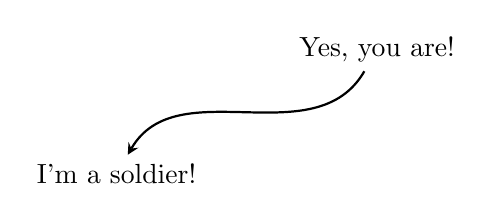
\begin{tikzpicture}[node distance=1.5cm]
		\node (test){I'm a soldier!};
		\node (testDesc)[above right=of test]
		{Yes, you are!};
		\draw [->,thick](testDesc)
		to[in=60,out=-120](test);
		\end{tikzpicture}
\end{codeshow}

在这里,我们引入了tikz宏包,以及它的positioning库,用来绘制和定位nodes。在 tikzpicture中,我们建立了两个\emph{node}: test和testDesc,后者的位于前者的右上方。最后,我们用绘制了从testDesc到test的曲线箭头,其样式由之前的\verb|\tikzset{>=stealth}|指定。

\begin{latex}

\end{latex}
